\chapter{Abläufe}
Im Folgenden werden die Interaktionen zwischen den Klassen und die internen Abläufe für alle wichtigen Testfälle in Form von Sequenzdiagrammen dargestellt. \\
Da die Testfälle T10, T20, T120, T130, T140, T150, T170, T180, T190, T200, T210, T220, T230, T240, T250 bereits von Airflow ohne unsere Erweiterungen erfüllt werden, werden hierfür keine Sequenzdiagramme benötigt. %T150 wie handelt code-editor das erstellen von neuen dags?

\begin{figure}[ht]
    \centering
    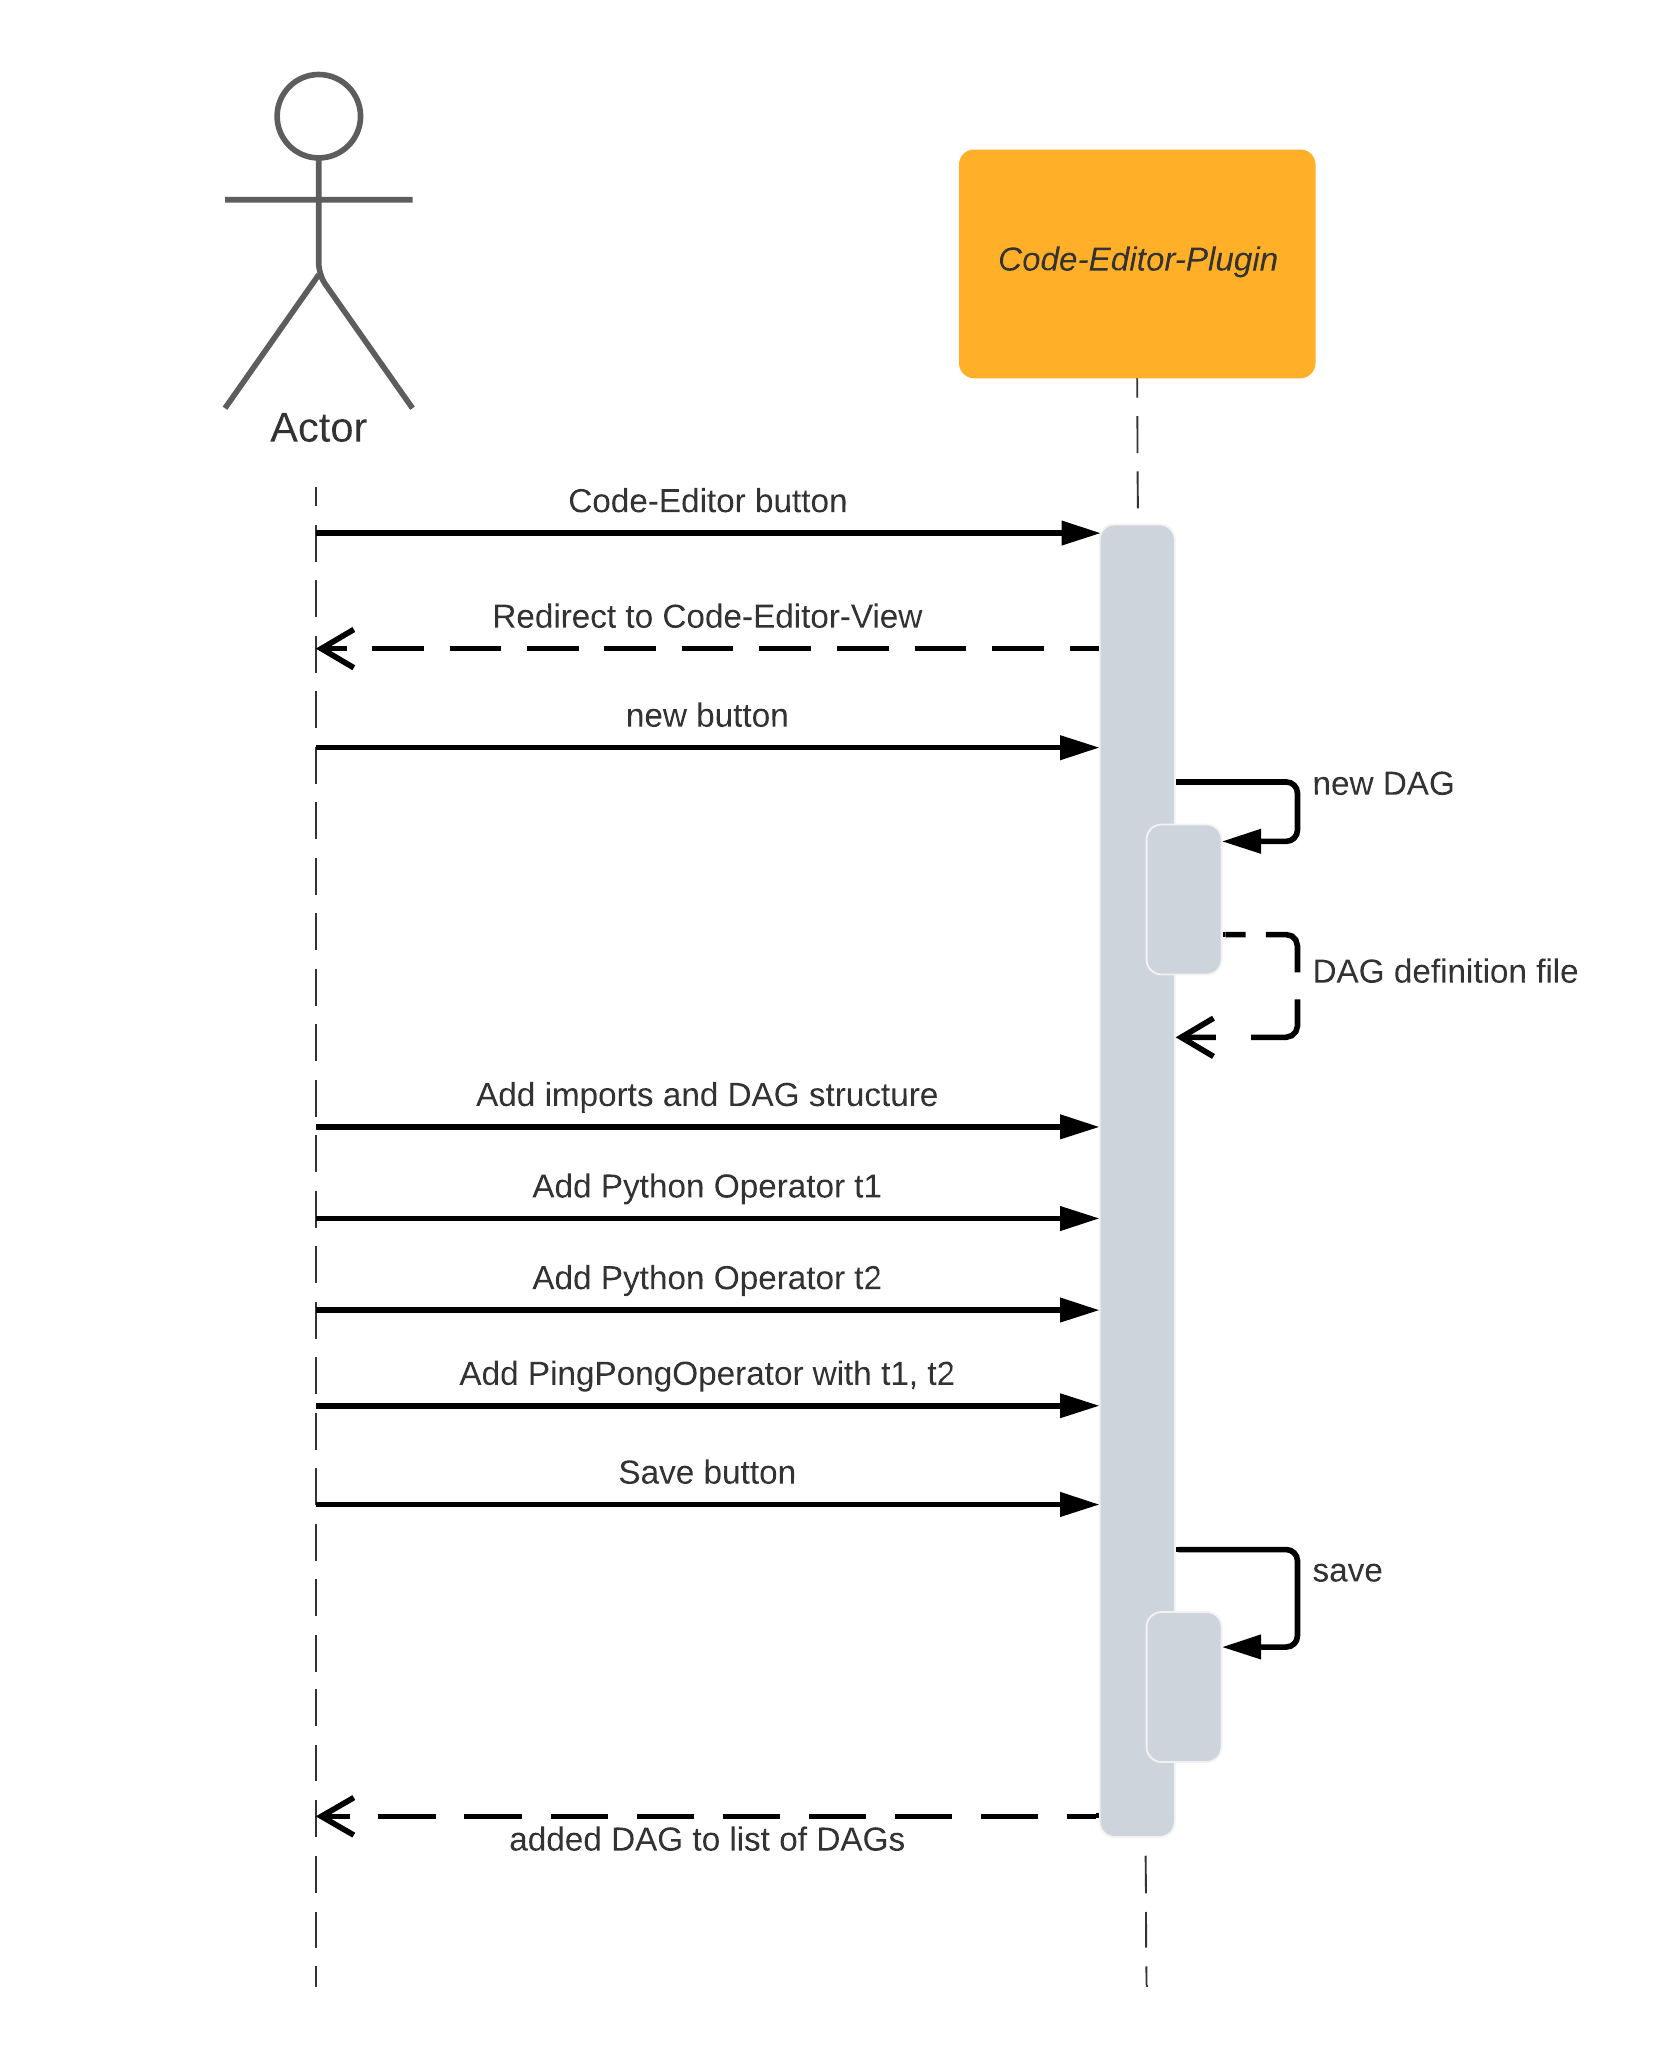
\includegraphics[width=0.95\textwidth]{Diagramme/Sequenzdiagramm T30.png}
    \caption{Sequenzdiagramm zum Testfall T30 zum Erstellen eines neuen Workflows.
    Diese Funktion wird vom Code-Editor-Plugin übernommen.}
    \label{fig:SQD_T30}
\end{figure}

\begin{figure}[ht]
    \centering
    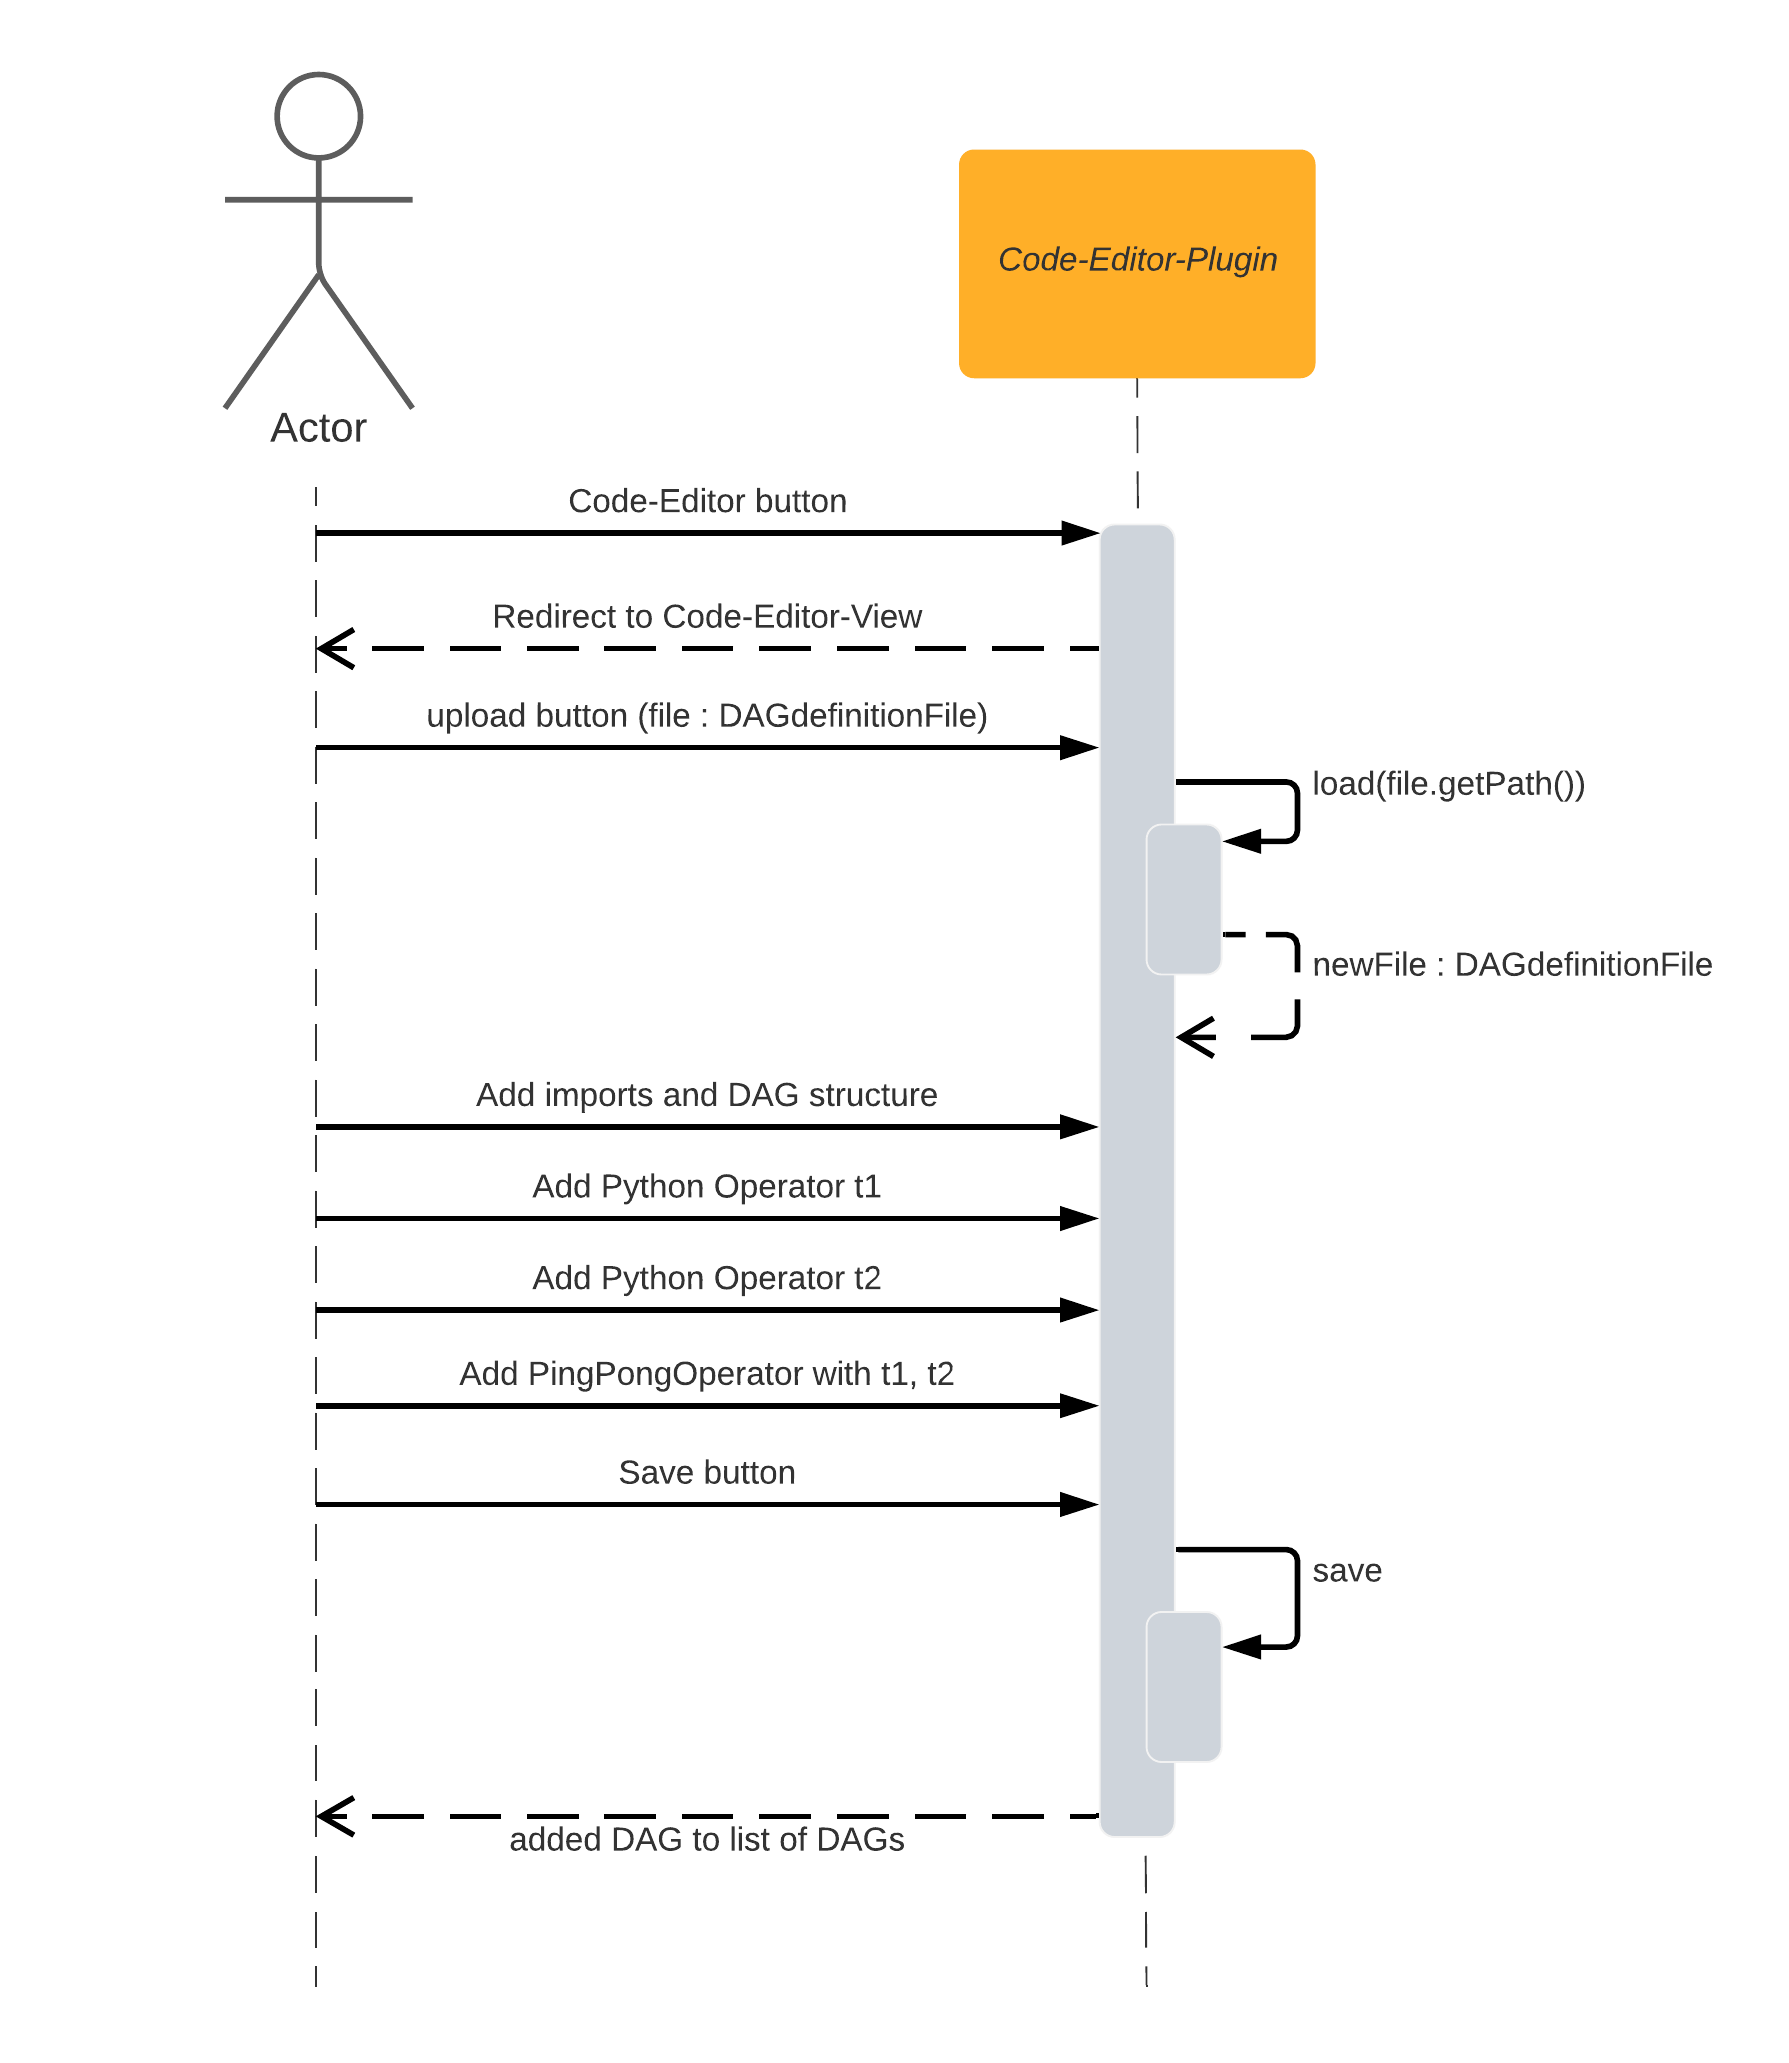
\includegraphics[width=\textwidth]{Diagramme/Sequenzdiagramm T9.png}
    \caption{Sequenzdiagramm zum Testfall T90 zum Importieren von Workflows. Diese Funktion wird vom Code-Editor-Plugin übernommen.}
    \label{fig:SQD_T90}
\end{figure}

\begin{figure}[ht]
    \centering
    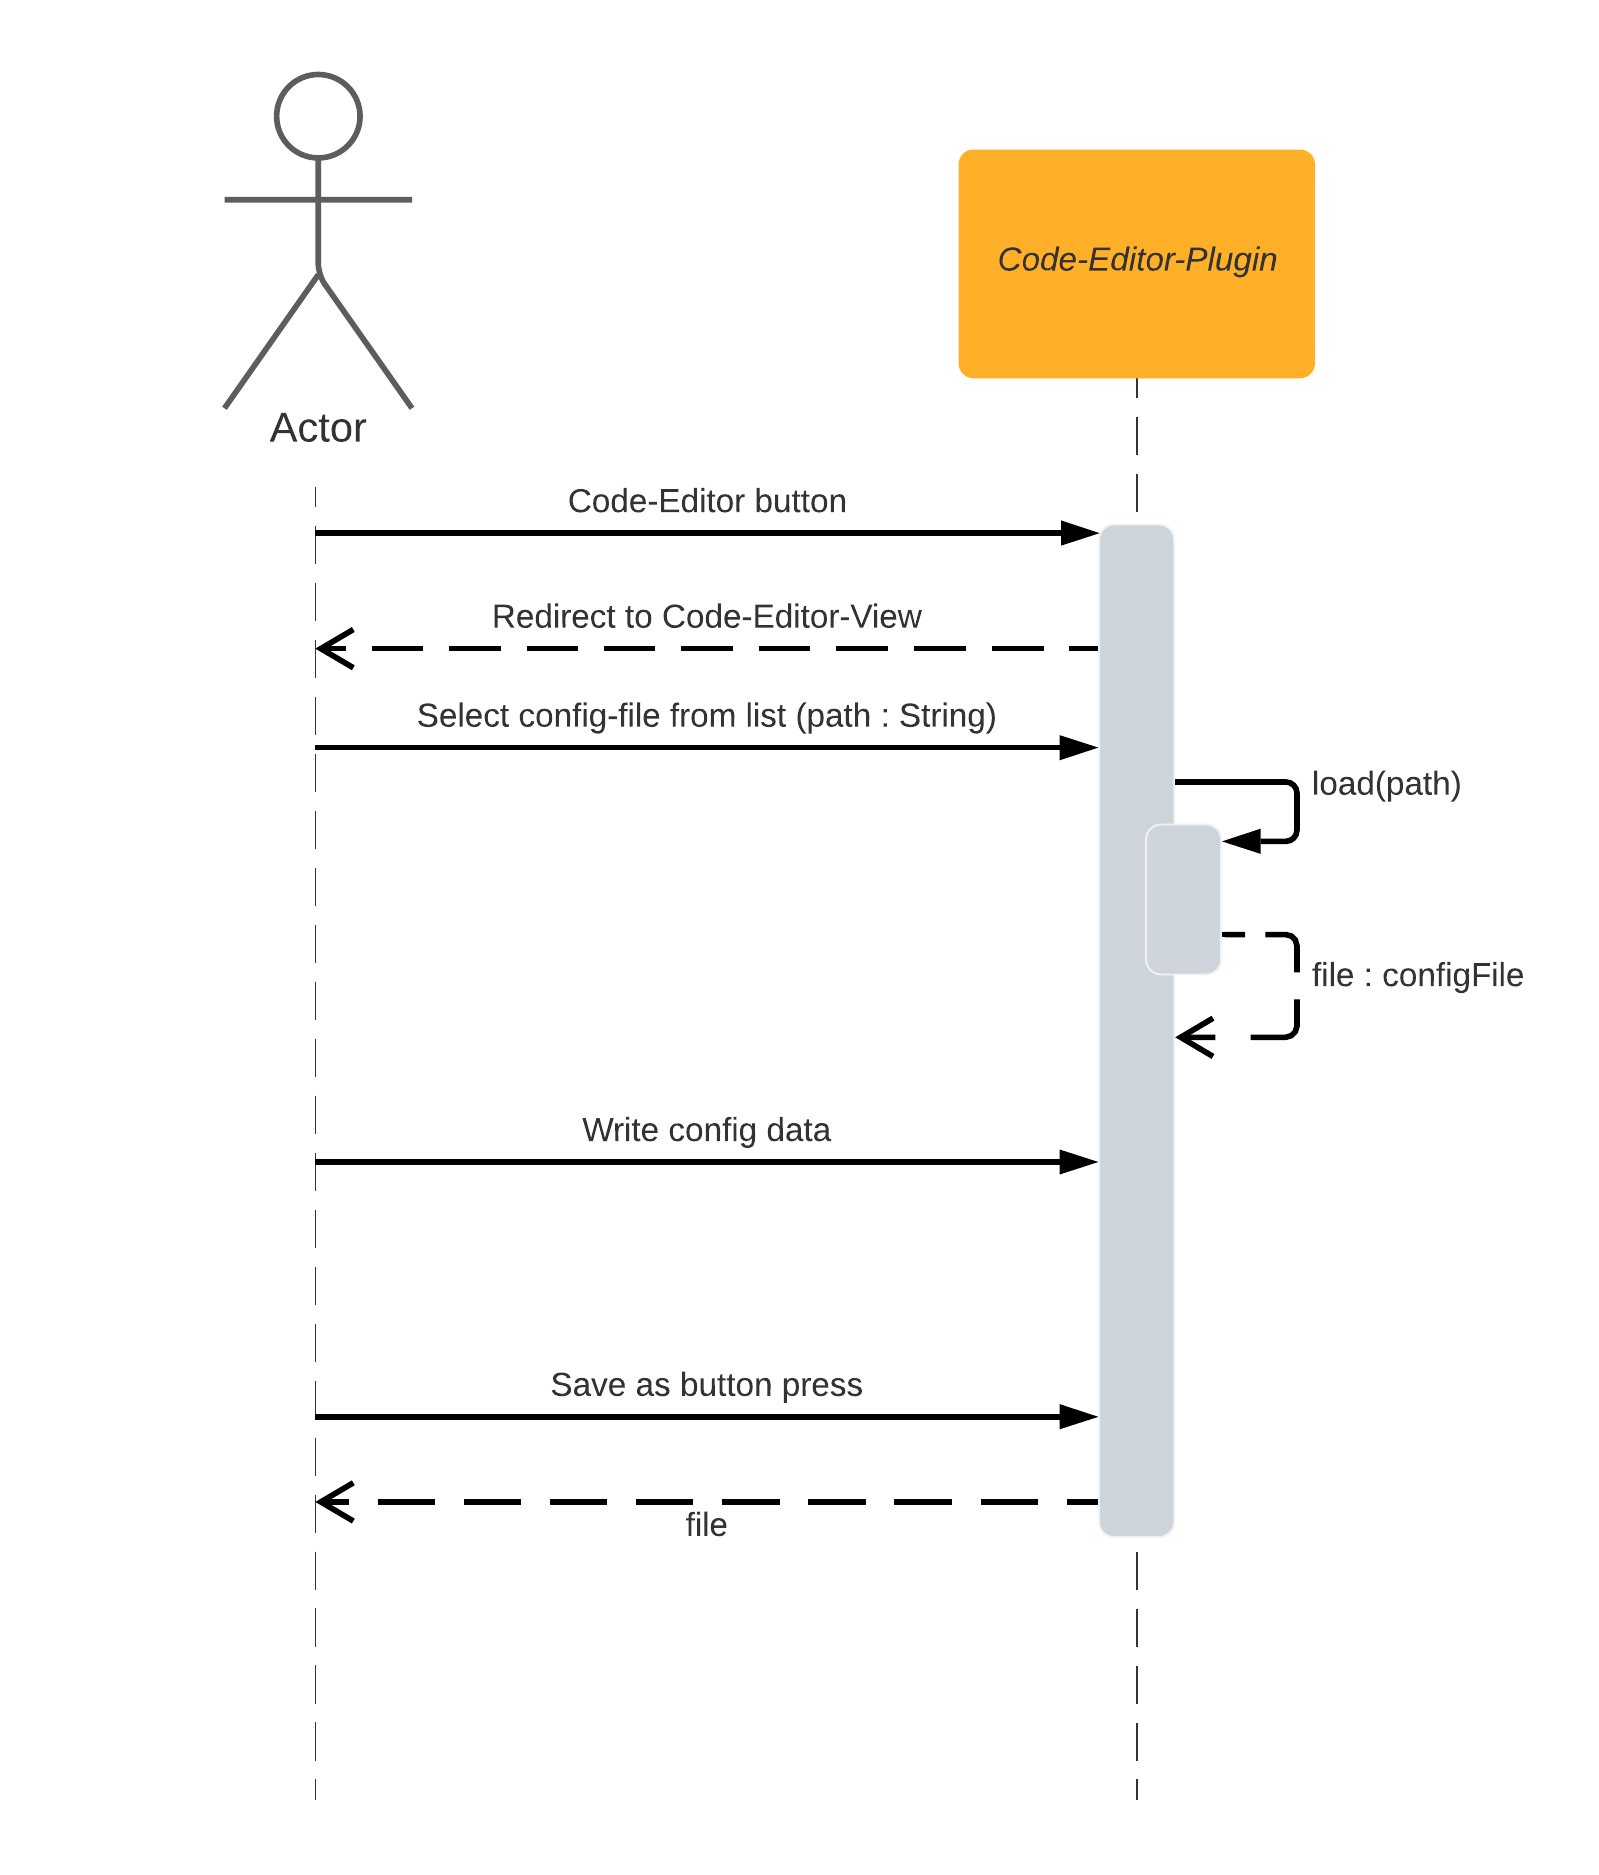
\includegraphics[width=0.9\textwidth]{Diagramme/Sequenzdiagram T100.png}
    \caption{Caption}
    \label{fig:SQD_T100}
    \caption{Sequenzdiagramm zum Testall T100 zum Bearbeiten einer Konfigdatei. Diese Funktion wird vom Code-Editor-Plugin übernommen.}
\end{figure}

\begin{figure}[ht]
    \centering
    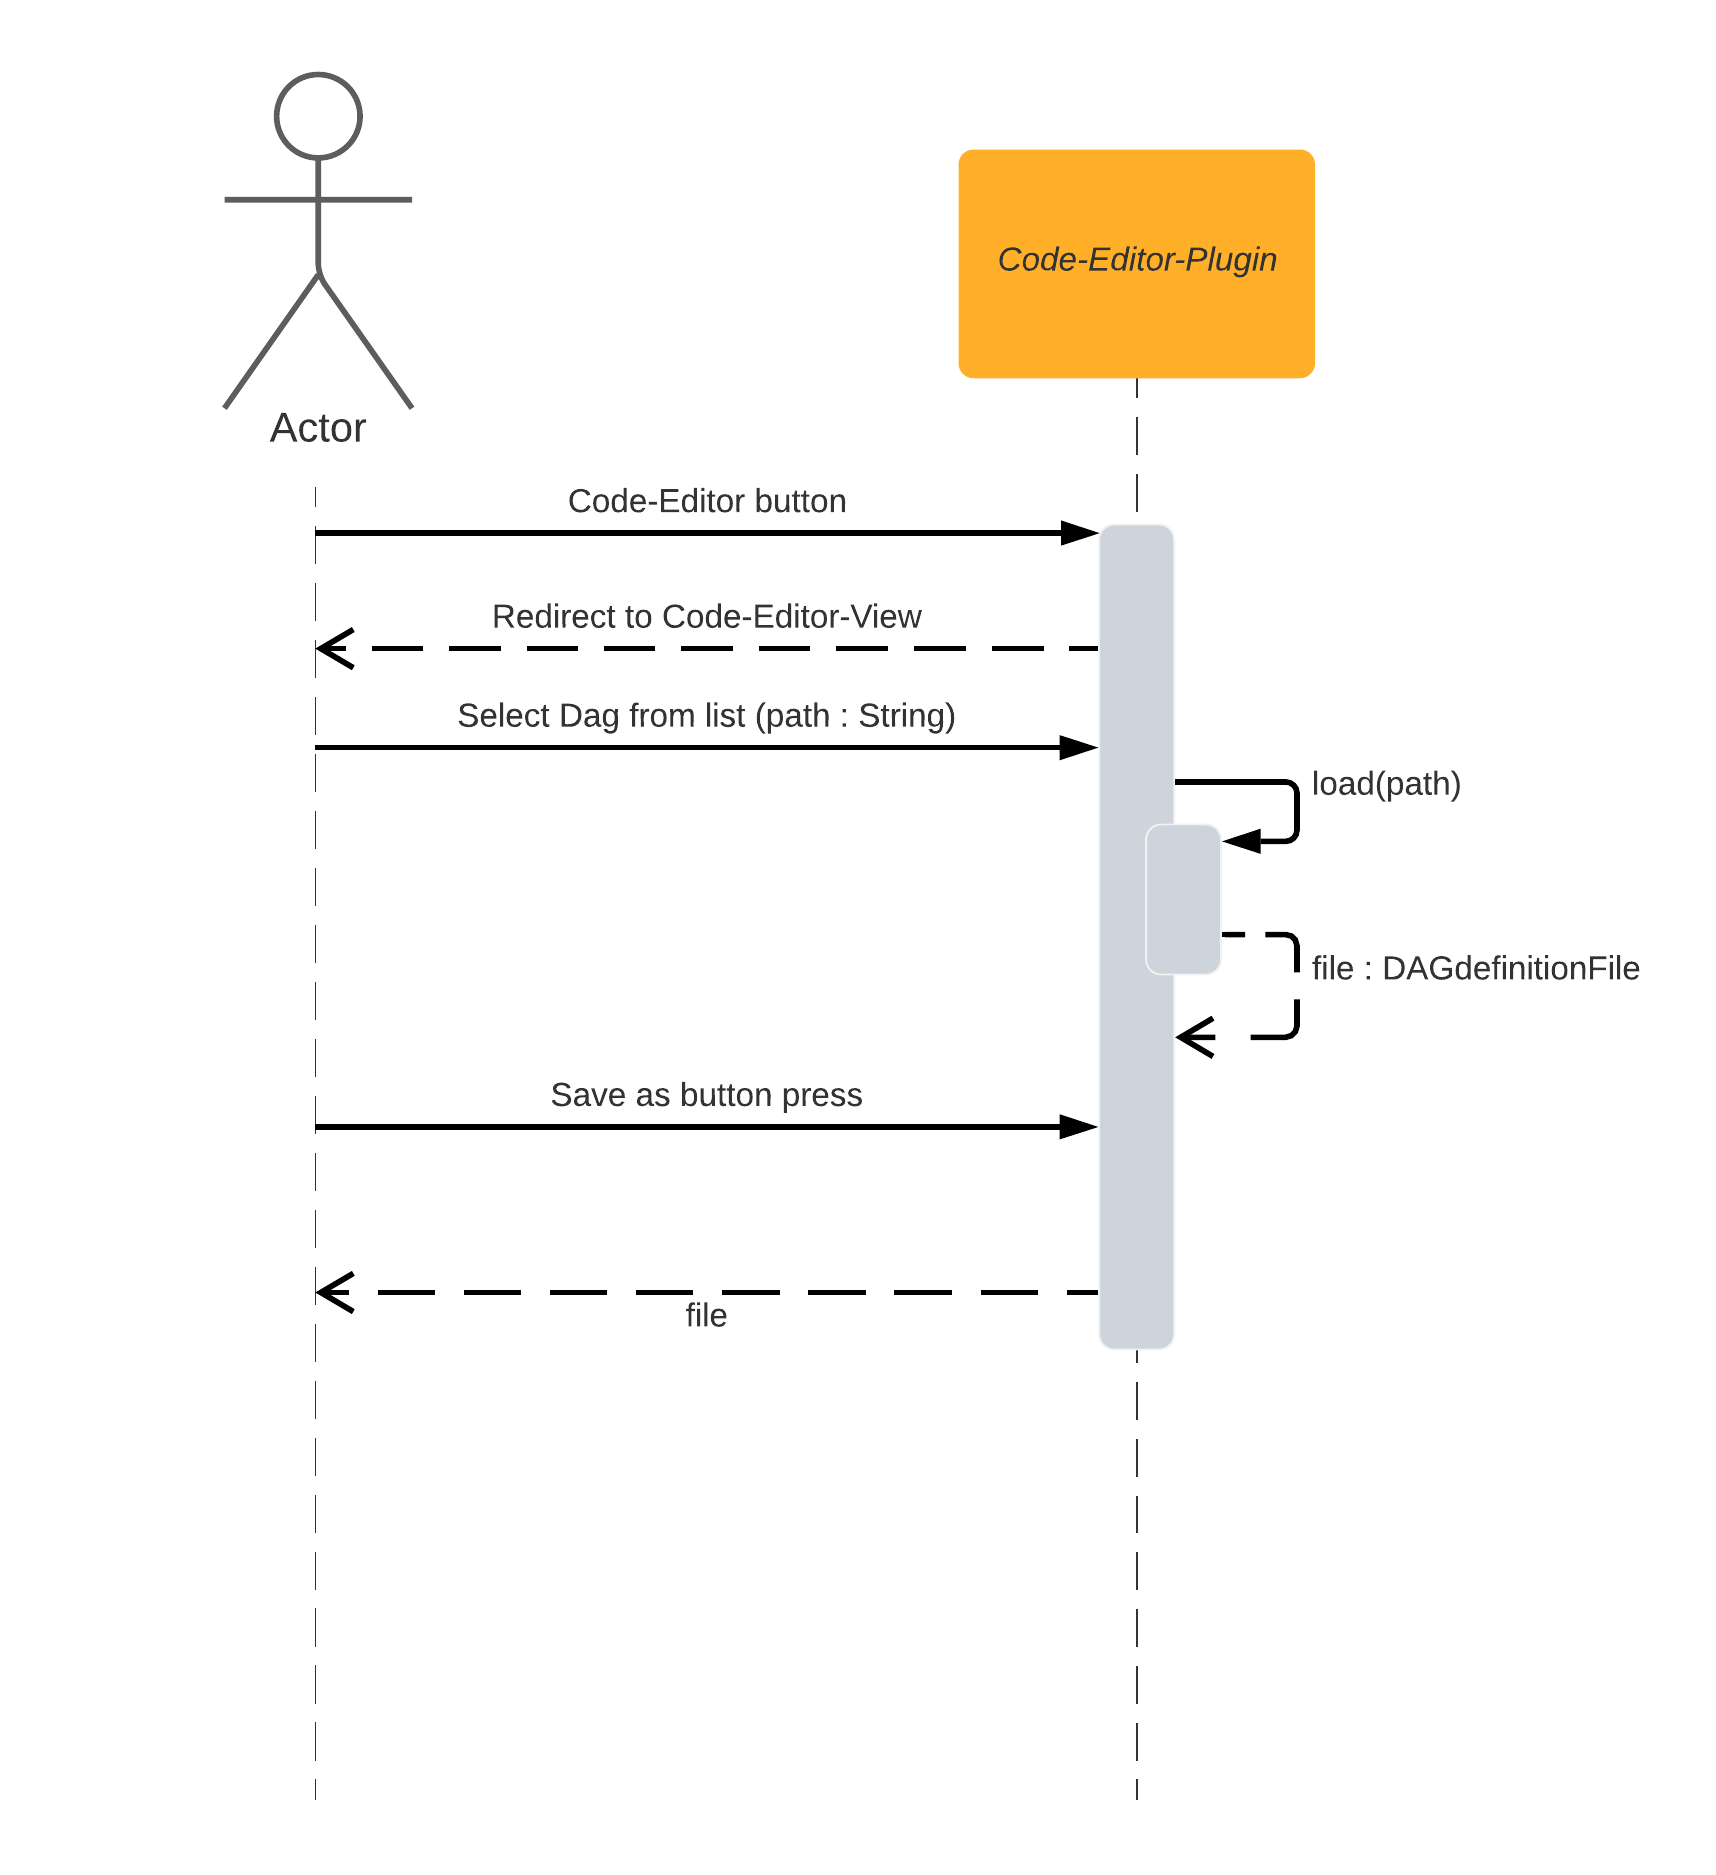
\includegraphics[width=\textwidth]{Diagramme/Sequenzdiagram T50.png}
    \caption{Sequenzdiagramm zum Testfall T50 zum Exportieren von Workflows}
    \label{fig:SQD_T50}
\end{figure}

\begin{figure}[ht]
    \centering
    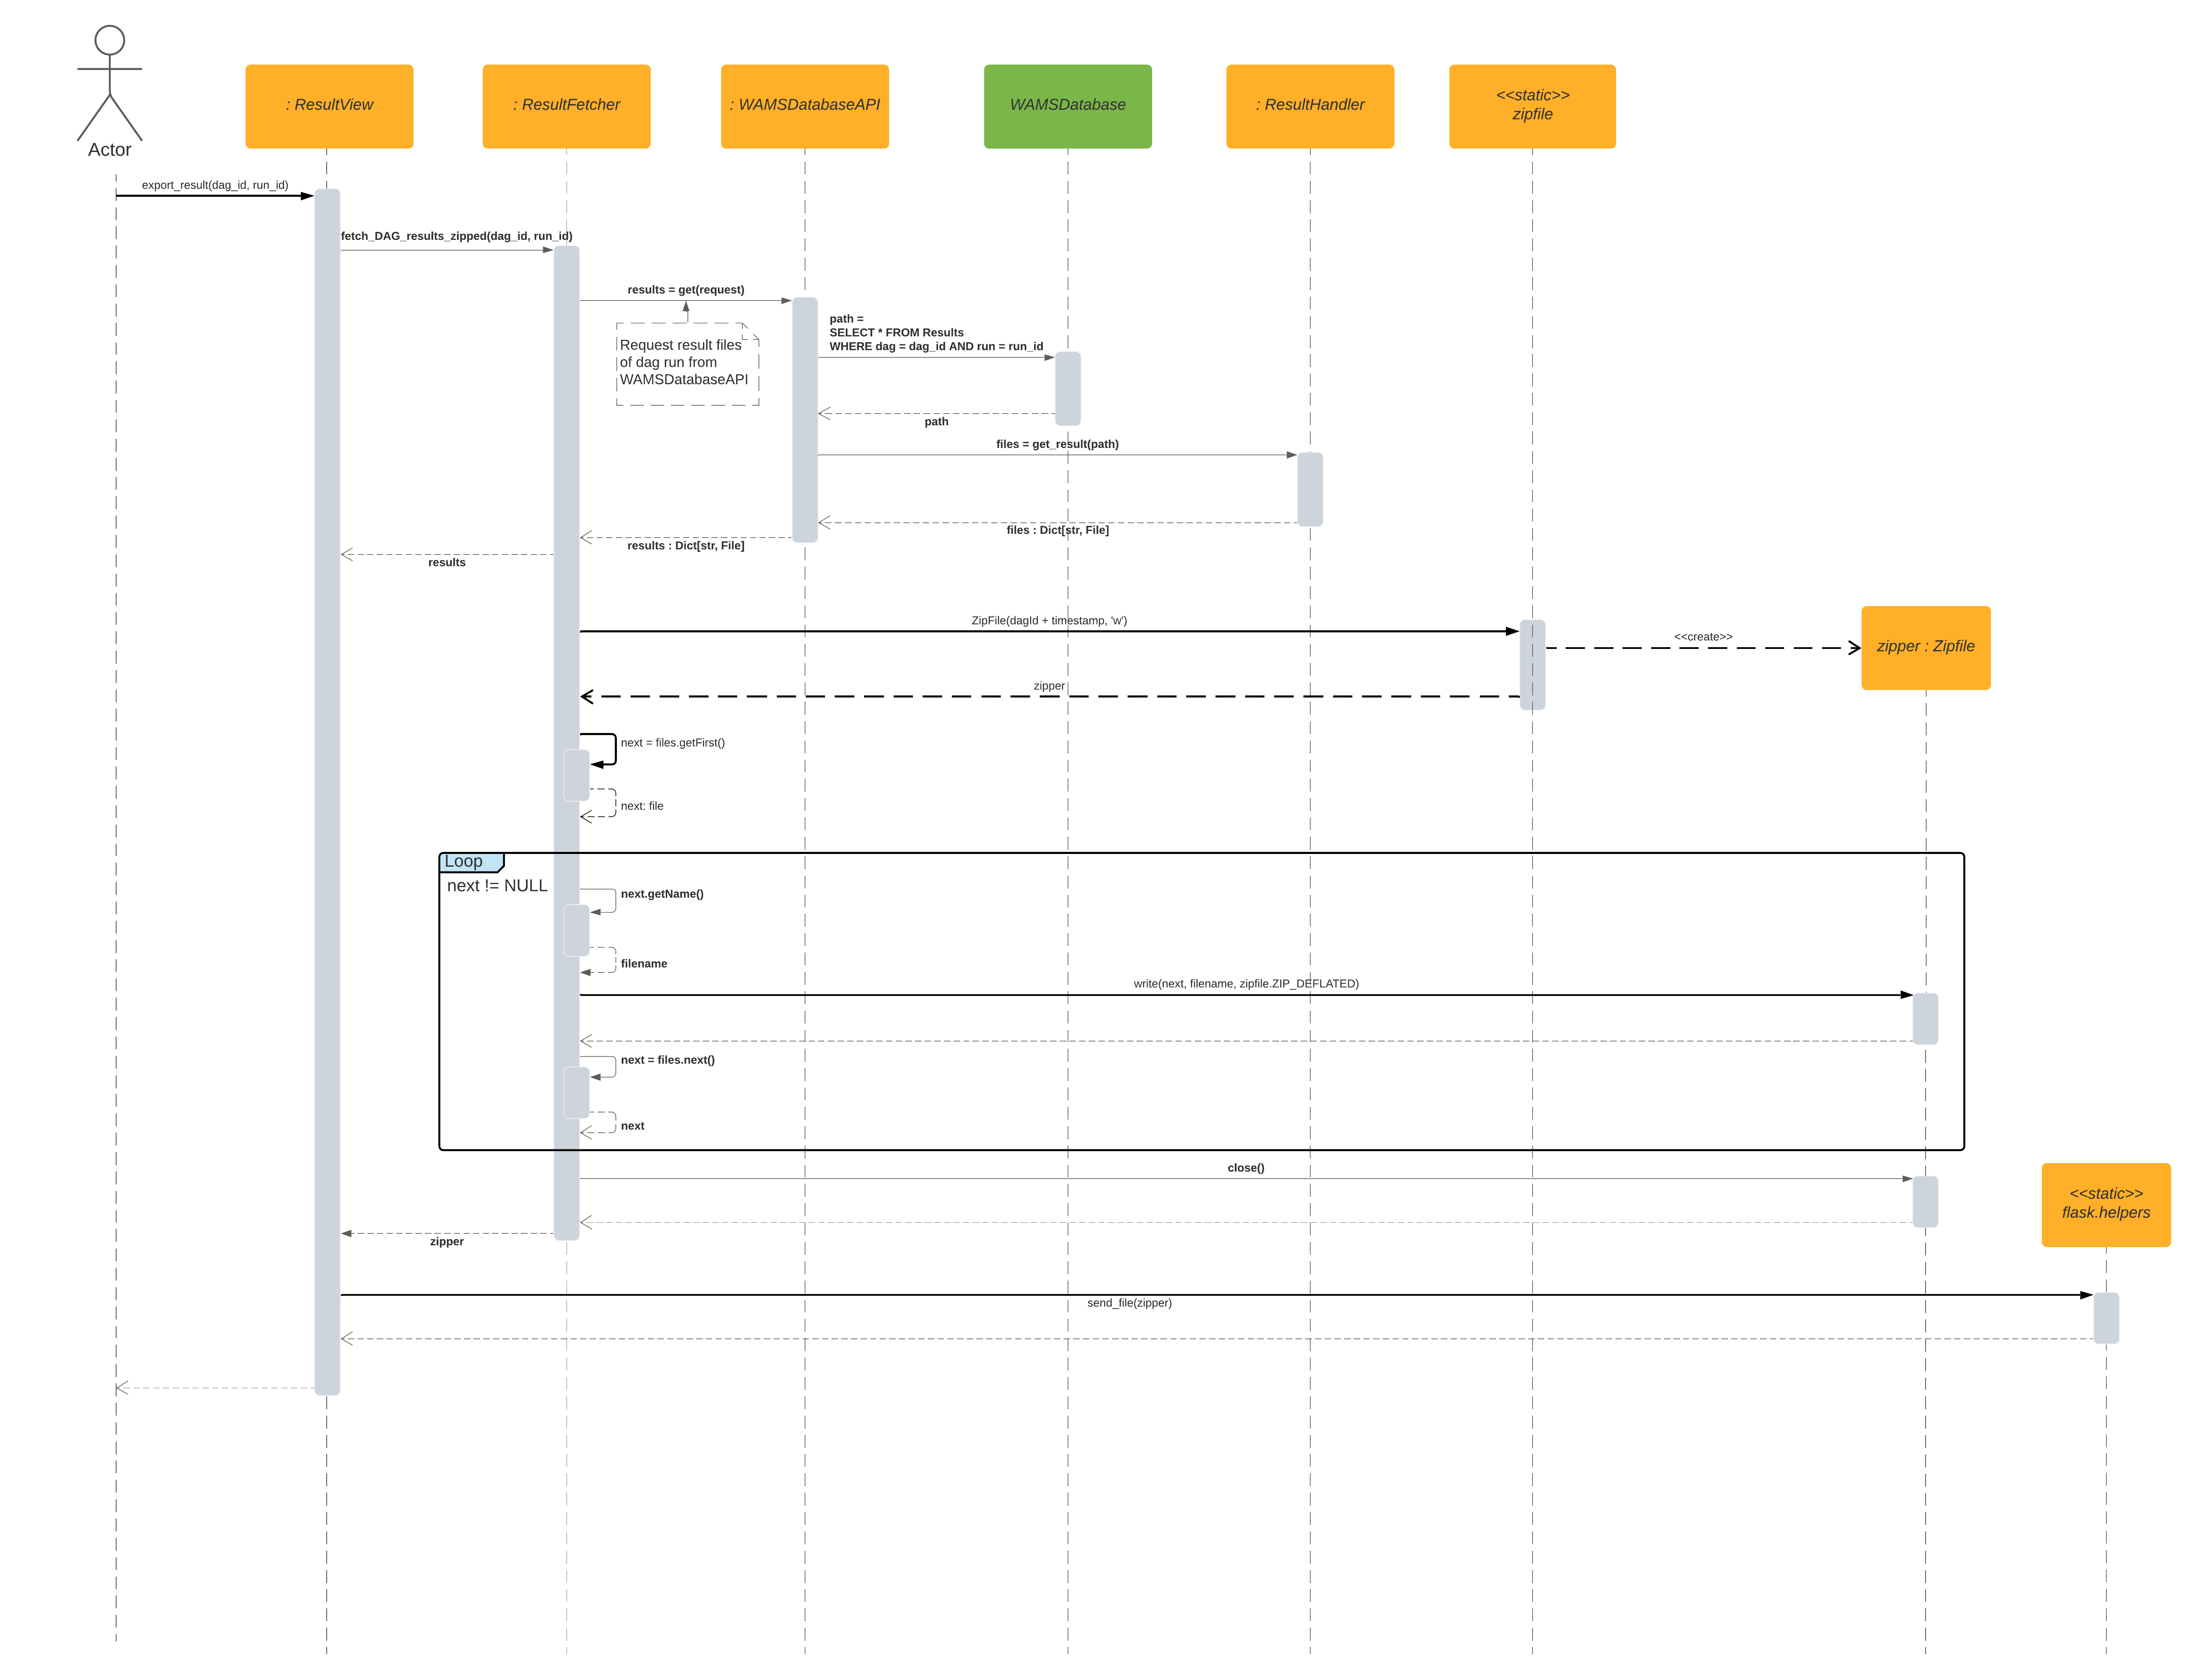
\includegraphics[width=\textwidth]{Diagramme/Sequenzdiagramm T110.png}
    \caption{Sequenzdiagramm zum Testfall T110 zum Herunterladen von Daten einer abgeschlossenen Workflorkflowinstanz}
    \label{fig:SQD_T110}
\end{figure}

\begin{figure}[ht]
    Aufgrund der Änderung von Testfall T60 zu einer Kombination der Testfälle T50 und T110, wird  für T60 kein eigenes Sequenzdiagramm benötigt.
    \label{fig:T60}
\end{figure}

\begin{figure}[ht]
    \centering
    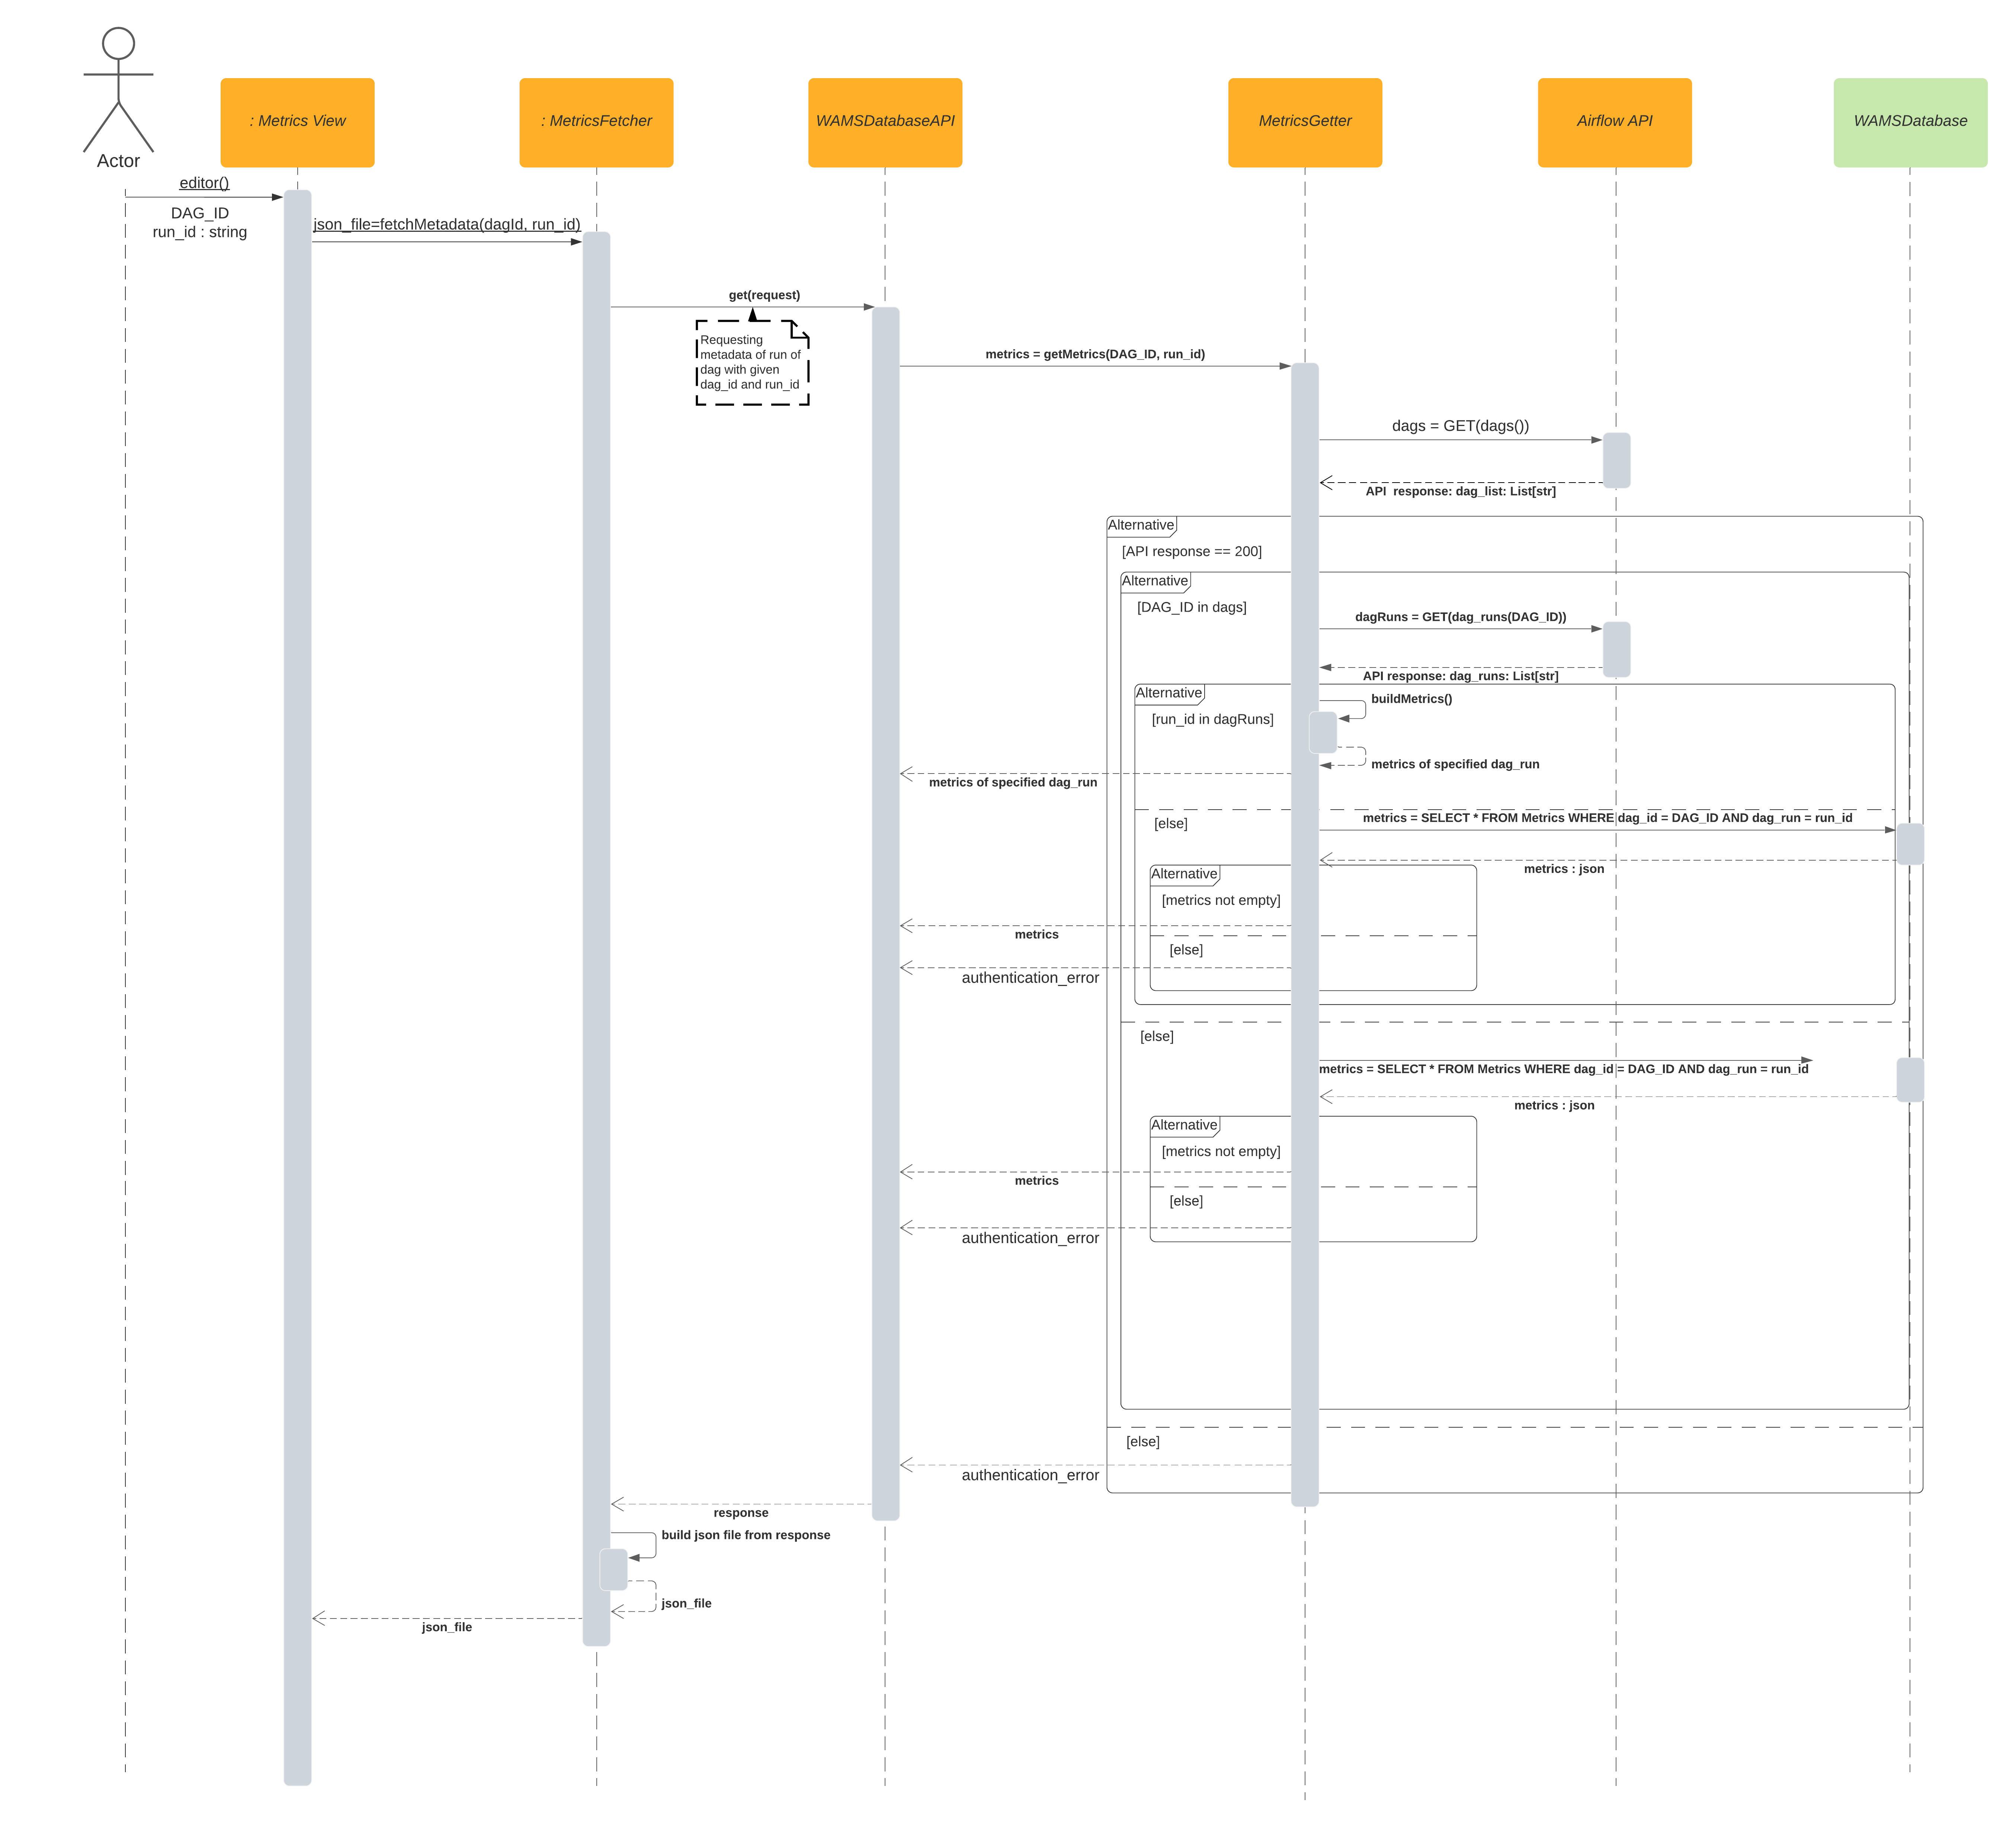
\includegraphics[width=0.97\textwidth]{Diagramme/Sequenzdiagramm MetadataFetcher.png}
    \caption{Sequenzdiagramm zum Anzeigen von Metadaten einer Workflowinstanz}
    \label{fig:SQD_MetadataFetcher}
\end{figure}



% Sequenzdiagramm fertig:
%T30 Workflow anlegen 
%T90 Workflow importieren 
%T50 export 
%T110 Daten von abgeschlossener WFI herunterladen 
%T60 
%T100 Workflow konfiguration bearbeiten 

% Könnte von Airflow übernommen werden wenn die Formulierung anders wäre:
%T40 fällt weg
%T60
%T160 noch nicht gestartete Instanz löschen fällt weg

%Sequenzdiagramm wird benötigt und Formulierung im Pflichtenheft ändern:
%T70 Instanz info einsehen <-- Noch zu besprechen


%Keine Funktion bisher:
%T80 Workflow umbenennen













%